\section{Overall Description}\label{intro}
\subsection{Product perspective}
\subsubsection{Scenarios}
\begin{enumerate}[label=\textbf{\Alph*}.]
    \item  \textbf{Educator Registration} \\
    Marco, un docente presso l'Università di Napoli, ha recentemente scoperto la piattaforma CKB grazie a un collega. Interessato alle sue potenzialità nel migliorare le competenze di sviluppo software degli studenti, Marco ha deciso di iscriversi come educatore. Visitando la home page di CKB, ha selezionato l'opzione "Registrati" e inserito il suo indirizzo email, scelto una password e fornito nome e cognome. Dopo aver inserito queste informazioni, è stato richiesto a Marco di verificare la sua email cliccando su un link inviatogli per garantire la sicurezza del suo account. Una volta completata questa verifica, ha proseguito con la registrazione selezionando l'opzione "Iscriviti come educatore". Con la registrazione completata con successo, Marco è stato reindirizzato alla sua dashboard personale all'interno di CKB, dove ha avuto accesso a una panoramica delle funzionalità per educatori, inclusa la possibilità di creare nuovi tornei e battaglie.
\item  \textbf{Student Registration} \\
Andrea, uno studente dell'Università di Bologna, ha scoperto l'applicazione CKB grazie al consiglio del suo professore. Affascinato dall'opportunità di affinare le sue competenze di sviluppo software attraverso sfide di code kata, Andrea ha deciso di iscriversi alla piattaforma. Una volta sulla home page di CKB, ha selezionato l'opzione "Registrati" e fornito il suo indirizzo email, creando una password. Ha anche inserito il suo nome e cognome, scegliendo l'opzione "Iscriviti come studente" per completare la registrazione. Tuttavia, prima di finalizzare il processo, il sistema ha richiesto a Andrea di verificare il suo indirizzo email cliccando su un link inviatogli, per assicurare l'autenticità del suo account. Durante questo passaggio, Andrea ha ricevuto un messaggio di errore: l'indirizzo email era già presente nel sistema di CKB. Ha prontamente corretto l'indirizzo email, utilizzando un account valido. Una volta verificata con successo la sua email e completato il processo di registrazione, Andrea è stato reindirizzato alla sua dashboard personale su CKB. Qui, ha potuto esplorare le varie funzionalità disponibili per gli studenti, come i tornei attivi, le competizioni imminenti e le informazioni sui suoi progressi nella piattaforma.
    \item \textbf{Tournament Creation} \\ 
    Daniele, professore di informatica presso il Politecnico di Milano, desidera creare un torneo sulla piattaforma CKB per permettere ai suoi studenti di sviluppare e migliorare le loro competenze di programmazione attraverso la partecipazione a battaglie di code kata.

Daniele accede alla piattaforma utilizzando le sue credenziali di accesso come professore e naviga alla sezione dedicata alla creazione di tornei sulla piattaforma CKB.

Successivamente, avvia il processo di creazione di un nuovo torneo selezionando l'opzione appropriata dalla dashboard principale. Il sistema richiede a Daniele di inserire  informazioni sul torneo, come il nome, una data di scadenza per la registrazione al torneo da parte degli studenti e la lista di colleghi che possono creare battaglie all'interno di tale torneo.

Il professore completa il modulo e, dopo aver inserito  le informazioni richieste, conferma la creazione del torneo. Il sistema verifica la validità delle informazioni fornite e, nel caso il nome del torneo risulti già esistente,  invierà il seguente warning:
"Il nome del torneo è gia esistente".
Altrimenti, in caso di verifica positiva, il sistema registra il nuovo torneo all'inteno del sistema. 
Tutti gli  studenti iscritti alla piattaforma ricevono notifiche sulla creazione del nuovo torneo.

\item \textbf{Battle Creation} \\ 
Giovanni, un professore  con privilegi di creazione di battaglie all'interno del torneo "Algorithms and data structures" sulla piattaforma CKB, decide di creare una nuova battaglia. A tale scopo,dopo aver effettuato l'accesso, naviga alla sezione dedicata alla creazione di battaglie e avvia il processo di creazione di una nuova battaglia. Il sistema richiede a Daniele di inserire informazioni essenziali sulla battaglia, tra cui una breve descrizione testuale, il progetto software con gli script di automazione della build, il numero minimo e massimo di studenti per gruppo, la data di scadenza per la registrazione e per la consegna del progetto.
Inoltre Daniele imposta informazioni aggiuntive che andranno ad incidere sulla valutazione del punteggio, come sicurezza, mantenimento e affidabilità. Infine, il sistema integra la nuova battaglia nella piattaforma. Gli studenti iscritti al torneo pertinente ricevono notifiche riguardo alla prossima battaglia.
\item \textbf{Tournament registration} \\
Sarah, una studentessa  di ingegneria informatica, si ritrova desiderosa di una nuova sfida per elevare le sue abilità di programmazione. Decide allora di collegarsi alla piattaforma CKB. Dopo aver effettuato l'accesso, esplora nella sezione dedicata ai tornei disponibili e ne individua uno in particolare - "Python  Challenge". Sarah clicca sul torneo e legge la sua descrizione e nota che la data di scadenza per la registrazione non è terminata. Senza esitazione, decide di partecipare alla Python Challenge. Cliccando su 'Iscriviti al torneo' Sarah riceve un messaggio di conferma e  fa ufficialmente parte del torneo. A questo punto può visualizzare tutte le battaglie in programma all'interno del torneo e verrà anche notificata alla creazione di battaglie future
.
\item \textbf{Battle registration} \\
Leonardo, studente iscritto al torneo "Super Tournament" su CKB, riceve una notifica che cattura la sua attenzione: "Chiamata alla Battaglia - Python Coding Challenge". Volentoroso di mettere alla prova le sue abilità di programmazione, Leonardo, dopo aver effettuato l'accesso, entra nella sezione dedicata alla battaglia, legge con attenzione i dettagli forniti e decide di iscriversi alla battaglia cliccando su "Iscriviti alla battaglia". Successivamente la piattaforma permette a Leonardo di scegliere se partecipare individualmente o invitare altri colleghi a formare un team per la battle, rispettando il numero minimo e massimo di partecipanti consentiti. Dopo la scadenza della fase di registrazione, la piattaforma CKB genera automaticamente una repository dedicata per il progetto della "Python Coding Challenge". Successivamente, il link diretto alla repository viene consegnato ai membri del team e reso disponibile nella sezione "Le tue battaglie" dell'applicazione.
\item  \textbf{Face the battle} \\
Il team "CodeCrafters", composto da appassionati studenti desiderosi di immergersi nella battle, riceve tramite mail il link alla repository su GitHub dedicata alla sfida "Algoritmi Avanzati" su CKB. Con un semplice click, procedono con il fork di tale repository, contenente il codice kata, dando così vita al loro spazio di lavoro virtuale. Per garantire una valutazione continua e precisa del loro lavoro, i CodeCrafters configurano GitHub Actions, che assicura una tempestiva comunicazione con la piattaforma.
Immersi nella stimolante sfida degli "Algoritmi Avanzati", i CodeCrafters avviano il processo di sviluppo adottando l'approccio test-first. Con creatività, creano le prime implementazioni, le sottopongono a test e le committano nella repository principale, tracciando così ogni passo del loro iterativo percorso. Ogni push prima della scadenza della battaglia attiva la piattaforma, che valuta automaticamente gli aspetti funzionali e la tempestività del lavoro dei CodeCrafters. Successivamente, la piattaforma calcola e aggiorna il loro punteggio di battaglia, offrendo feedback in tempo reale sulla qualità del loro prezioso contributo.
\item \textbf{Ranking display} \\
Matteo, durante la sua partecipazione a una battaglia su CKB, accedendo alla sezione del Torneo e della battaglia d'interesse può monitorare in tempo reale la posizione della sua squadra attraverso una classifica dinamica. Al termine della battaglia, si trova di fronte a una fase di consolidamento, durante la quale l'educatore può decidere se assegnare un punteggio personale al progetto o affidarsi esclusivamente al punteggio automatico. Alla conclusione di questa fase, Matteo può consultare la classifica finale  recandosi nella sezione dedicata alla battaglia appena conclusa, ottenendo così una panoramica completa delle prestazioni della sua squadra.

Il punteggio ottenuto in questa specifica battaglia si somma a quelli accumulati nelle battaglie precedenti, contribuendo a formare il suo punteggio complessivo nel torneo. Matteo e tutti gli utenti hanno la possibilità di esplorare la classifica nella sezione dedicata al torneo stesso , accessibile a tutti gli utenti interessati.

Infine, una volta che l'educatore chiude definitivamente il torneo, Matteo e gli altri iscritti a CKB possono consultare la classifica finale del torneo sempre nella sezione relativa a quel torneo.

\item \textbf{Evaluates project} \\
Una volta scaduta la fase di sottomissione di una battaglia del torneo "Algoritmi Avanzati" su CKB, il Professore Bianchi, creatore della sfida, si prepara ad eseguire una valutazione manuale dei progetti presentati dai team partecipanti.Accede alla piattaforma, seleziona il torneo e la battaglia appena conclusa. All'interno dell'interfaccia, trova una lista completa dei progetti degli  studenti se è stata aggiunta la valutazione manuale in fase di creazione della battaglia.
Inizia esaminando attentamente il codice sorgente prodotto da ciascun team, analizzando gli aspetti che non possono essere completamente valutati in modo automatico.
Durante questa fase, il Professore Bianchi attribuisce un punteggio personale a ciascun team in base alla sua esperienza e conoscenza approfondita, in particolare premiando la creatività, l'ingegnosità e l'approccio strategico dei team partecipanti. Terminata la valutazione lo score finale per ciascun team viene determinato facendo la media tra il punteggio assegnato manualmente dal Professore Bianchi e quello generato automaticamente dalla piattaforma.
\item \textbf{Tournament Closure}
Luisa, docente di informatica presso l'Università di Torino, ha gestito con successo il torneo "Logic Masters" sulla piattaforma CKB.Dopo l'ultima battaglia, decide di concludere il torneo.Luisa accede a CKB con le sue credenziali e naviga alla sezione del torneo "Logic Masters".Nella dashboard del torneo, trova l'opzione "Chiudi il Torneo".	Dopo aver cliccato selezionato tale opzione, appare un messaggio di warning: "Sei sicuro di voler chiudere il torneo?”.
Luisa deve scegliere tra "Conferma" per procedere con la chiusura o "Annulla" per annullare l’operazione. Con la conferma della chiusura, il sistema, se non vi sono ancora battaglie attive, chiude il torneo.
\end{enumerate}
\subsubsection{User interface}
The system needs to interact with users via devices that require an internet connection. To access the system, all users must connect through a web interface hosted on an existing domain, such as www.codekatabattle.com.
\subsubsection{Software interface}
The system will use some  external interfaces in order to accomplish its functionalities.
\begin{enumerate}
    \item The system is required to retrieve data from  database, necessitating the implementation of  interfaces to ensure accurate data retrieval.
    \item The system interacts with external APIs to offer email notification services.
    \item The system interacts with GitHub to create and manage repositories for code kata exercises. It sets up automated workflows using GitHub Actions to track code commits, trigger updates, and calculate battle scores.
\end{enumerate}
\subsubsection{Interfaccia Hardware}

CKB è accessibile da una varietà di dispositivi hardware, garantendo un'esperienza utente ottimale su diverse piattaforme. Di seguito sono elencati i principali dispositivi hardware supportati:

\begin{itemize}
    \item Computer Desktop e Laptop

    \item Smartphone e Tablet 

\end{itemize}






\subsection{Domain class diagram}
In the figure is represented the domain class diagram related to CKB. This diagram is used  to represent the key concept of our system and the interaction between them.
The main elements of the diagram are:
\begin{itemize}
    \item The 'User' class is responsible for representing users within the system. It is divided into two specialized subclasses: 'Educator' and 'Student.' This division allows for the more effective management of specific functionalities and behaviors for each type of user. Educators have the ability to create tournaments and battles within the system. Students have the opportunity to enroll in tournaments created by educators and participate in battles.
    \item The 'Tournament' class represents tournaments within the system. It possesses a crucial attribute known as 'Educator Permissions.' This attribute serves the purpose of indicating which educators have the authorization,given by the tournament's creator, to create battles within that specific tournament.
    \item  The 'Automated Evaluation' class represents an evaluation process that is automated and consistently carried out. It encompasses predefined parameters and criteria to assess specific elements automatically. Furthermore, 'Manual Evaluation' is a specialized form of evaluation within the system, and it extends from the 'Automated Evaluation' class. It shares the same predefined parameters and criteria as automated evaluation, but with the added capability of manual assessment by educators. Unlike automated evaluations, manual evaluations are not performed automatically but are initiated at the discretion of educators. Educators have the flexibility to decide whether to conduct a manual evaluation or not, enhancing the evaluation process when educator intervention is desired
\end{itemize}

\begin{figure}[h] % [h] indica che LaTeX dovrebbe cercare di posizionare l'immagine qui, ma potresti utilizzare anche altre opzioni come [htbp]
  \centering % Centra l'immagine orizzontalmente
  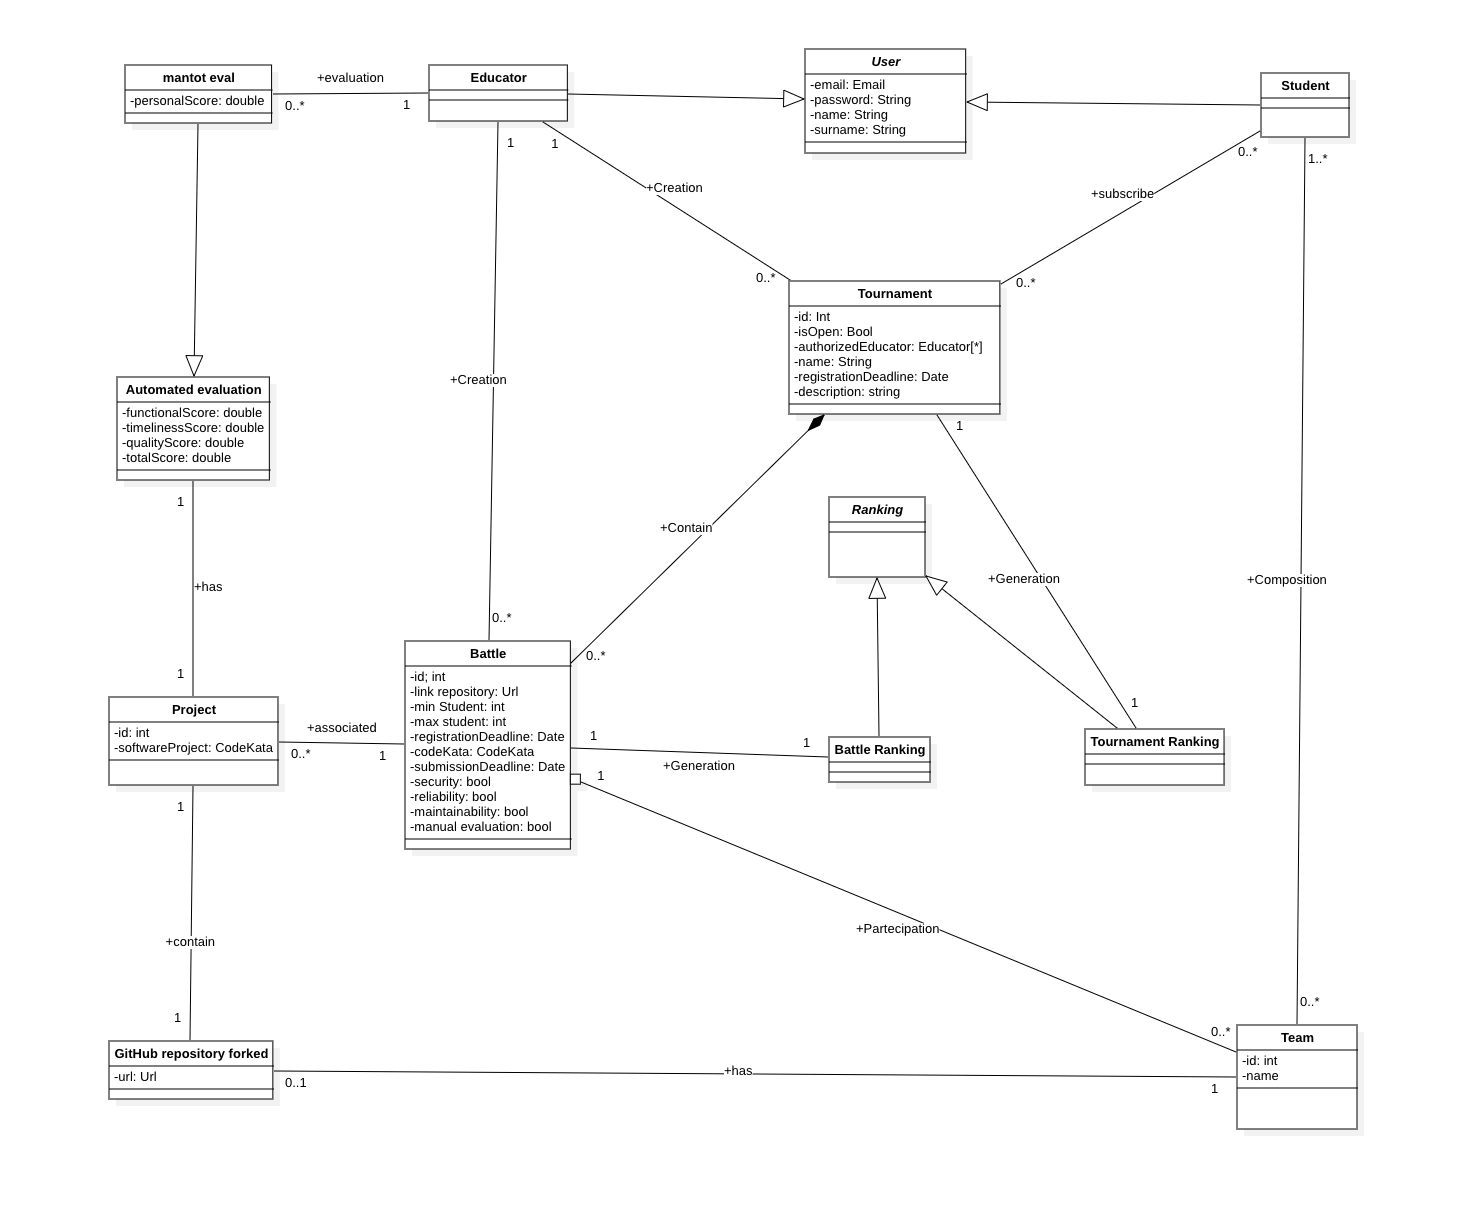
\includegraphics[width=0.95\textwidth]{ClassDiagram.png} % Sostituisci "nomefileimmagine" con il nome del tuo file immagine
  \caption{Descrizione dell'immagine} % Aggiungi una didascalia all'immagine
  \label{fig:etichetta} % Aggiungi un'etichetta per riferimenti futuri
\end{figure}




\subsection{StateChart Diagrams}
Lo StateChart Diagram è un diagramma utilizzato per descrivere il comportamento di classi in termini di stato. Il diagramma mostra gli stati che sono assunti  dalla classe in risposta ad eventi esterni.

    \begin{figure}[H]
  %\centering
  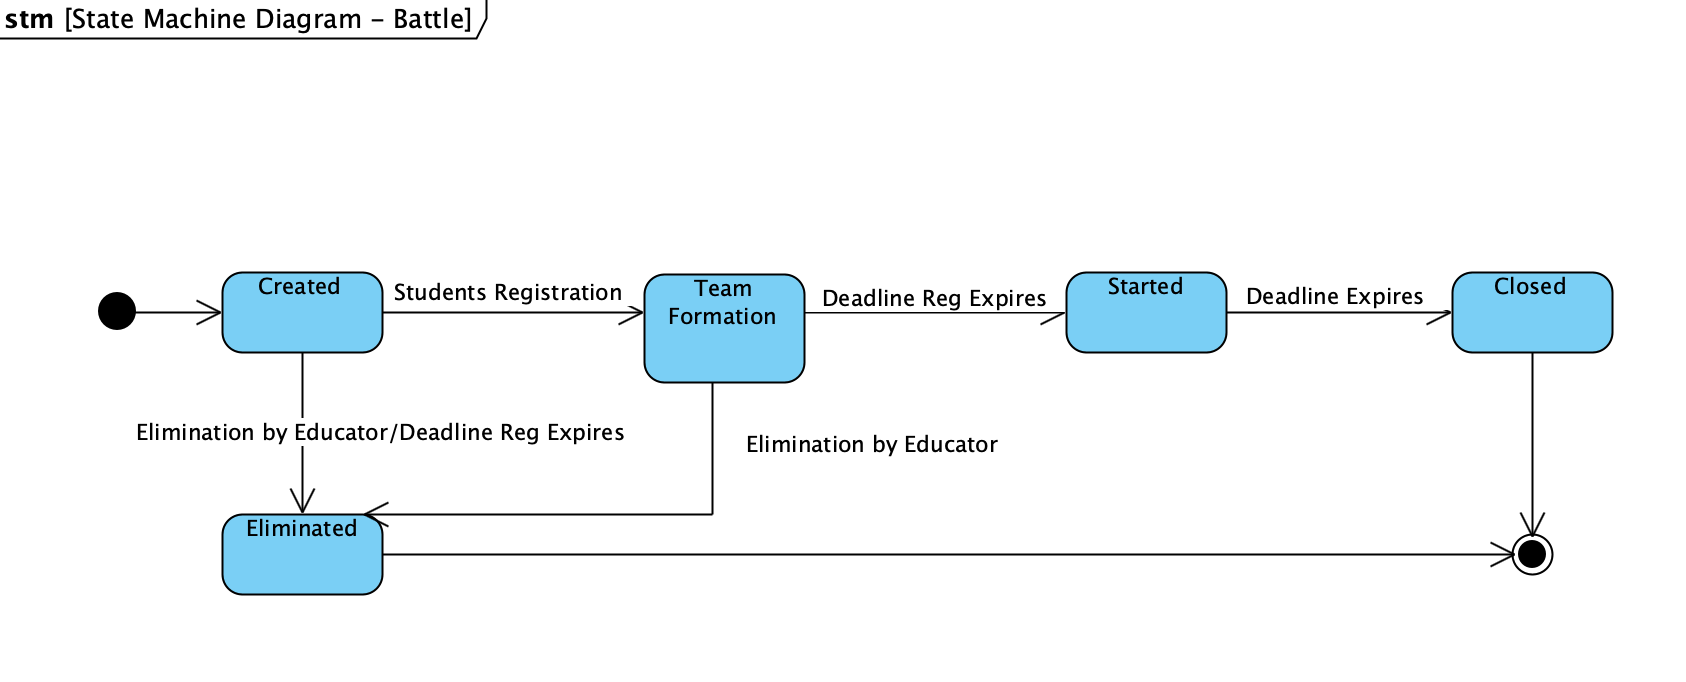
\includegraphics[width=1\linewidth]{StateChart/BattleStateChart.png} 
  \caption{Didascalia dell'immagine}
  \label{fig:immagine}
\end{figure}
    \begin{figure}[H]
  %\centering
  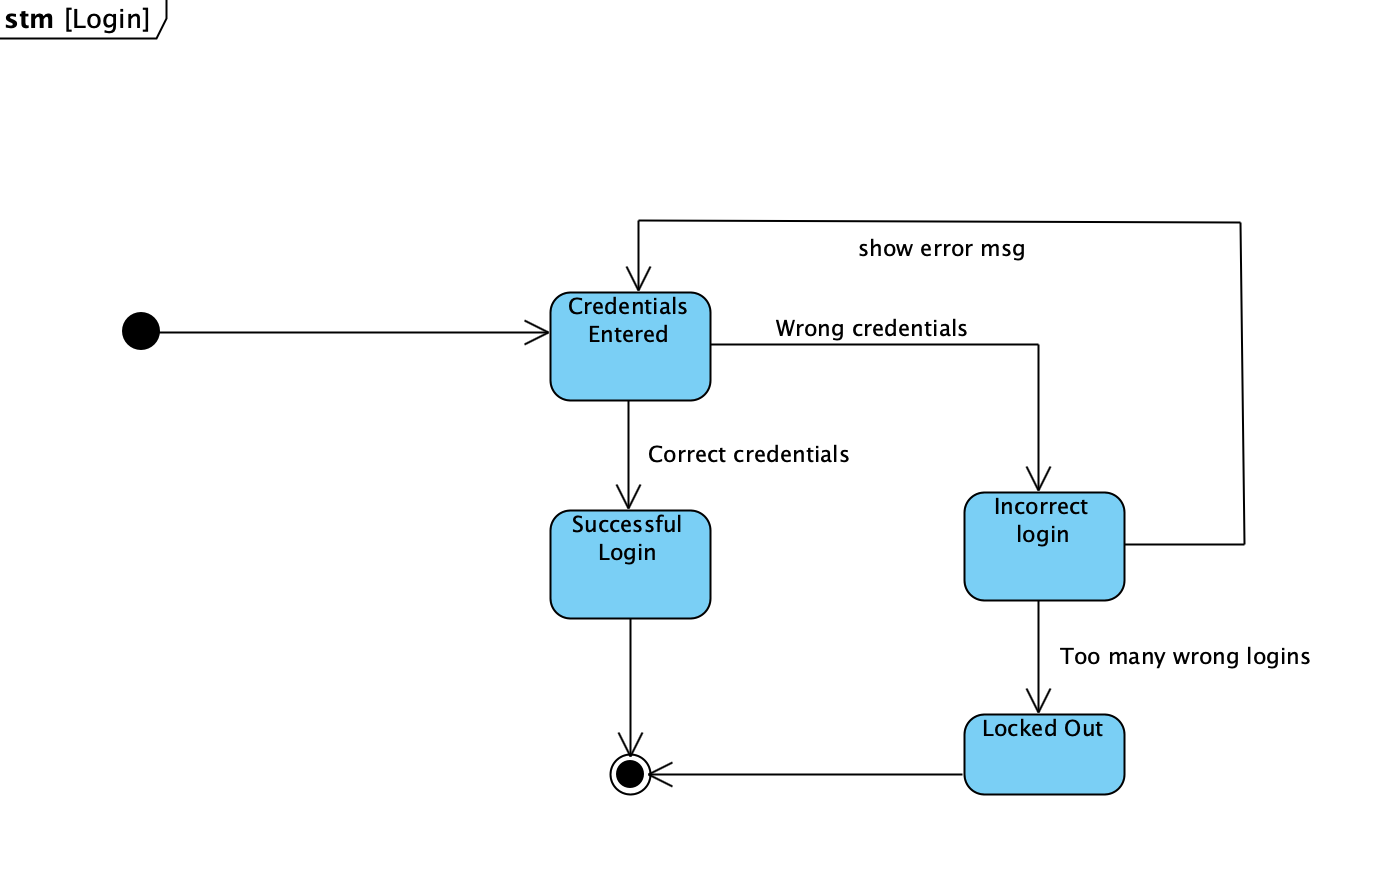
\includegraphics[width=1\linewidth]{StateChart/LoginStateChart.png} 
  \caption{Didascalia dell'immagine}
  \label{fig:immagine}
\end{figure}
    \begin{figure}[H]
  %\centering
  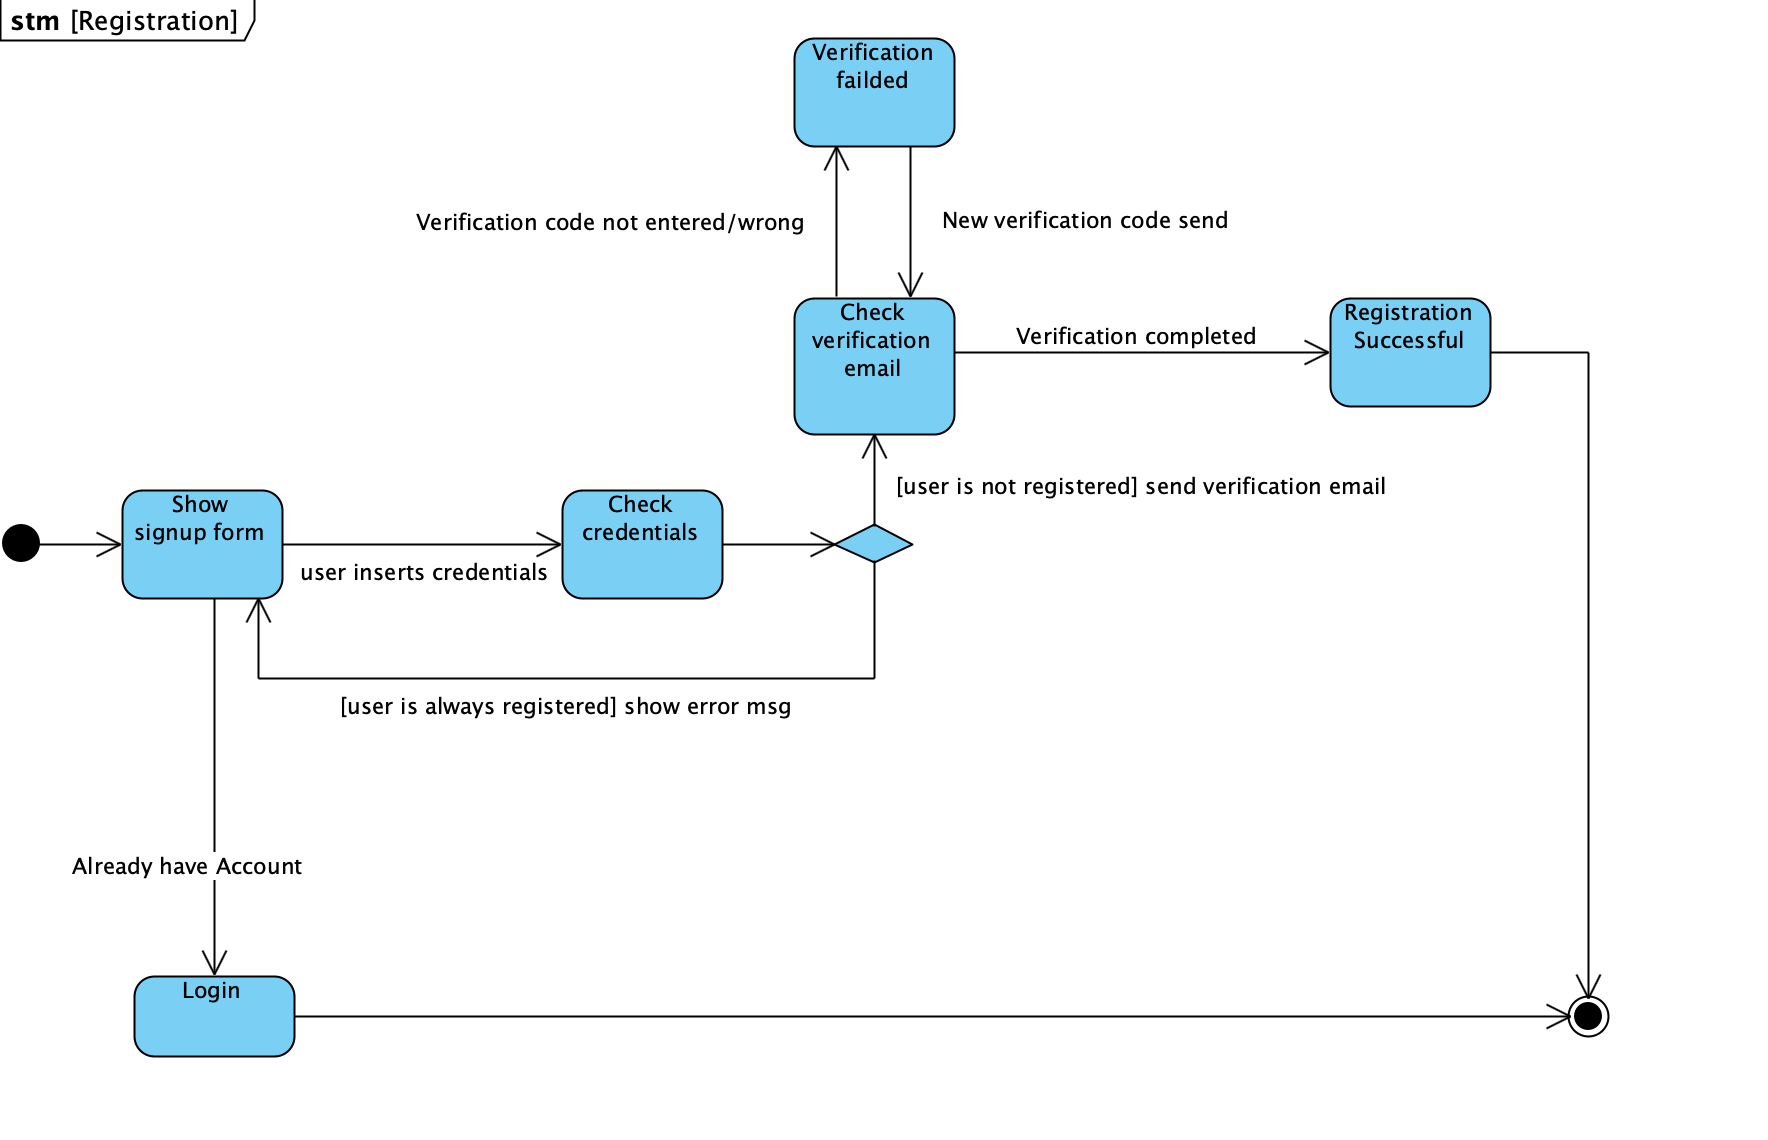
\includegraphics[width=1\linewidth]{StateChart/RegStateChart.png} 
  \caption{Didascalia dell'immagine}
  \label{fig:immagine}
\end{figure}
    \begin{figure}[H]
  %\centering
  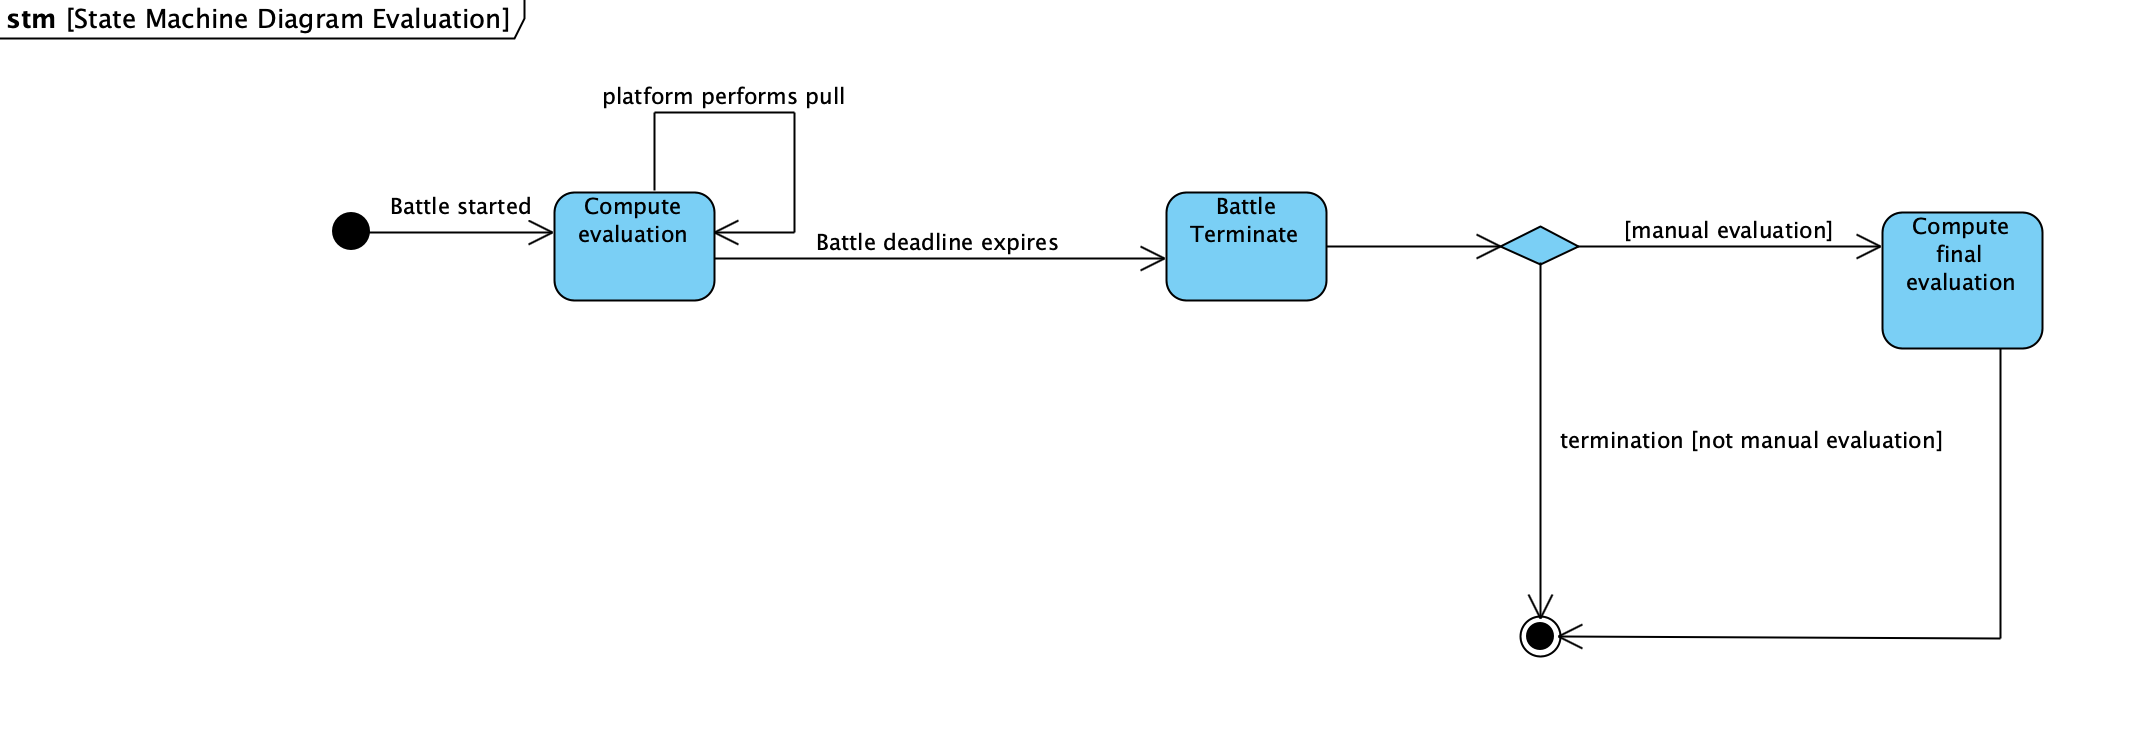
\includegraphics[width=1\linewidth]{StateChart/EvaluationStateChart.png} 
  \caption{Didascalia dell'immagine}
  \label{fig:immagine}
\end{figure}

\newpage

\textbf{Evaluation process}



\noindent The diagram outlines a process initiating with the 'Compute evaluation' stage. At this stage, following the commencement of a battle, the platform conducts an automated assessment of the projects. Every time pull operations are performed to obtain the latest code updates submitted by students through GitHub pushes, the system reverts to the 'Compute evaluation' stage for a fresh assessment.
This is followed by the 'Battle deadline expires' transition, indicating the end of the project submission deadline and that no new commits for evaluation are accepted.

\noindent Next, the process moves to the 'Battle Terminate' state, marking the end of the battle. Here, all automatic scores have been assigned, and no further contributions are accepted.

\noindent If a 'manual evaluation' is set, the process can diverge towards a manual evaluation. In this case, if the educator needs to manually assess the students' work, the process proceeds to the 'Compute final evaluation' state. The educator reviews the projects, assigns a manual score which is added to the automatic score to determine the final score of the battle. Otherwise, without a manual evaluation, the process concludes, relying solely on the automatic evaluation for the final score.


\textbf{Battle Lifecycle }


\noindent The Statecharts diagram illustrates the flow of events for a code kata battle within the CKB platform. The battle begins with the "Created" state, indicating the initiation of a new challenge by the educator. In this phase, if no students sign up before the registration deadline or if the educator decides to cancel the battle, it transitions to the "Eliminated" state, leading to the removal of the battle from the platform. However, if at least one student signs up, it proceeds to the "Team Formation" state, where students have the opportunity to form teams. After the registration deadline, it enters the "Started" state, marking the actual commencement of the battle, allowing students to start working on their code projects. This state persists until the final submission deadline. Finally, the "Closed" state represents the conclusion of the battle.
\subsection{Product Functions}
This section provides  a summary of the major functions that the software will perform.\\

\begin{itemize}
    \item A general user can:
    \begin{itemize}
        \item Register
         \item Login
    \end{itemize}
\item A student can:
    \begin{itemize}
    \item Subscribe to a tournament
    \item Subscribe to a battle
    \item Form a team for the battle
    \item Explore the ranking of battles/tournaments
    \end{itemize}
\item  An educator can:
\begin{itemize}
    \item Create a tournament
    \item Create a battle
    \item Give permission to create battle within his tournament to other educators
    \item Manually evaluate student's projects.
\end{itemize}
\end{itemize}
\subsection{User characteristics}
As we have seen in the class diagram, there are two type of users: student and educator.
\subsubsection{Student}
A student is defined as someone eager to learn and enhance their programming skills. Students can navigate through dedicated pages on the CKB site to select the tournaments they are most interested in. They have the opportunity to participate in individual challenges or form teams, depending on the specific rules of each battle. In doing so, they compete with other students registered on the platform, testing their abilities and knowledge.
\subsubsection{Educator}
Anyone who wishes to create tournaments and battles, incorporating engaging and challenging tasks, is considered an educator. An educator has the freedom to upload various types of software projects within a battle, thus allowing anyone who registers to participate and compete. Moreover, educators have the ability to grant permissions to other educators to create battles within their tournaments. They also have the option to personally evaluate the tournament results or rely on the platform's default automated evaluation system.
\subsection{Assumptions, dependencies and constraints}

\subsubsection{Assumptions}
These assumptions represent properties and/or conditions that the system takes for granted, primarily because they are beyond the control of the system itself. It is necessary to verify them to ensure the correct behavior of CKB.
\label{sec:assumptions_dependencies_and_constraints}%
\newcounter{da}
\setcounter{da}{0}
\newcommand{\cda}{\stepcounter{da}\theda}
\begin{center}
    \begin{longtable}{ |l|p{0.9\linewidth}| }
        \hline
        \textbf{ID} & \textbf{Description}                                                                                     \\
        \hline
        DA\cda      & Both educators and students must have an e-mail.                                         \\
         \hline
        DA\cda      & Students must have a  Github account.                                         \\
        \hline
        DA\cda      & Users who register on the CKB platform in the role of 'educator' are skilled  in designing meaningful and challenging code katas and also in evaluating them.                                                                           \\
        \hline
        DA\cda      & Users have consistent and reliable access to the internet and the necessary technology (computers, software development tools) to participate in coding battles and tournaments.                                                       \\
        \hline
        DA\cda      & The integration with GitHub and GitHub Actions functions correctly, allowing for seamless repository management, code submission, and automated workflow for the students’ projects.                                  \\
        \hline
        DA\cda      & Users who register on the CKB platform in the role of 'student'  have familiarity with programming languages,  GitHub, and test-driven development methodologies.        \\
        \hline
        \caption{Domain assumptions.}
        \label{tab:domainassmptn_tab}%
\end{longtable}
\end{center}


\subsubsection{Hardware Constraints}
The system has to run under the following worst-case conditions:
\begin{itemize}
    \item Internet Connection: Minimum 5 Mb/s.
    \item Screen Resolution: 1024x768.
    \item Modern Web like
\end{itemize}

\subsubsection{Regulatory policy}
The CKB application requires users to provide personal details, including their first name, last name, and email address. We assure users that their email addresses will not be utilized for any commercial or marketing purposes. All personal data collected will be handled and processed in strict adherence to the General Data Protection Regulation (GDPR), ensuring the highest standards of privacy.

